\section{Some notes on OpenGL}
\label{opengl:opengl_notes}

One of the design target of OpenGL was to made its API portable 
among multiple architectures. In order to do so, OpenGL 
designers decided not to make use of polymorphism and inheritance 
when they had to provide multiple versions of the same command 
taking different parameters. They used, instead, the following scheme:

\begin{verbatim}
    glCommandName{NTd}()
\end{verbatim}

that is, every OpenGL function is preceded by \texttt{gl} and can be 
followed by

\begin{itemize}
  \item \texttt{N} \\
    the number of parameters the function takes
  \item \texttt{T} \\
    the parameters type
  \item \texttt{d} \\
    if present, it states that the function takes pointers as arguments
\end{itemize}

For example, the \texttt{glVertex} can be invoked as:

\begin{itemize}
\item \texttt{glVertex2i(1, 3)}
\item \texttt{glVertex2f(1.0, 3.5)}
\end{itemize}

As you might have observed from the simple example above,
OpenGL commands use the prefix `gl' and initial capital letters
for each word making up the command name (`glClearColor()', for
example). Similarly, OpenGL defined constants begin with `GL\_', use all
capital letters, and use underscores to separate words (for example,
'GL\_COLOR\_BUFFER\_BIT').
\\
You might also have noticed some seemingly extraneous letters appended to
some command names (for example, the `3f' in `glColor3f()' and `glVertex3f()').

\subsection{The Depth Buffer}
\label{opengl:opengl_note:depth_buffer}

When drawing up a scene with OpenGL, the order in which polygons are drawn
greatly affects the blended result, especially when it comes to 3D.
\\
The depth buffer keeps track of the distance between the viewpoint and 
the portion of the object occupying a given pixel in a window on the 
screen; when another candidate colour arrives for that pixel, it's drawn 
only if its object is closer to the viewpoint, in which case its depth
value is stored in the depth buffer. With this method, obscured (or hidden)
portions of surfaces aren't drawn and, therefore, aren't used for
blending.
\\
In order to enable the use of the depth buffer, the 
\texttt{glutInitDisplayMode()} can be used, passing the 
GLUT\_DEPTH macro as an argument.

\subsection{OpenGL viewing model}
\label{opengl:opengl_note:viewing_model}

OpenGL not only provides function to specify models for 
three-dimensional objects but also allows to specify the 
position for each of the models we want to display in a 
scene and also the point from which to view the scene.
\begin{figure}[!h]
  \begin{center}
    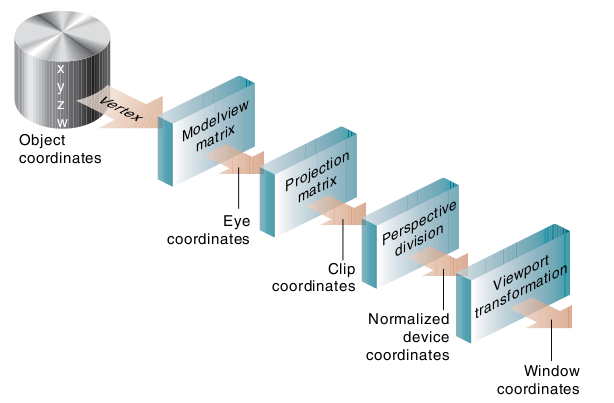
\includegraphics[width=300pt]{img/openGLpipe.png}
    \caption{The OpenGL pipeline}
    \label{fig:openglpipe}
  \end{center}
\end{figure}
\\
The transformation process used to produce a scene for viewing 
is analogous to taking a photograph with a camera (in fact, it 
is often addressed as \textit{the camera analogy} 
\cite{opengl:cameraanalogy}) 
and consists of four steps, known as
\textit{the OpenGL pipeline} (see figure \ref{fig:openglpipe}).
\\
At the beginning of the pipeline, we have the \textit{raw} 
coordinates of the models we want to put on the scene. Such 
coordinates are then multiplied by the a 4x4 \textbf{modelview} 
matrix, that is, a matrix that stores both \textit{model} and 
\textit{viewing} transformations and which elements have been set 
accordingly to \textit{actually} where to place items in the scene.
\\
The second step involves the \textbf{projection} matrix, 
which is applied to the incoming object coordinates to define a 
viewing volume. Of course, objects outside this volume are clipped 
so that they are not drawn in the final scene. 
\\
In the last two steps of the pipe, incoming coordinates are transformed 
into actual two-dimensional window coordinates and other stuff, such as 
the light intensity for each pixel, are calculated according to depth.

\subsection{Matrix transformations}
\label{opengl:opengl_note:matrix_transfor}

To edit the \textbf{modelview} and \textbf{projection} matrices, OpenGL 
provides quite a lot of functions: some of them are 
\textit{general purpose}, that is, they can be used to edit both of them, 
others are specifically intended to edit either the modelview or the 
projection matrix.
\\
The most used \textit{general purpose} functions are 

\begin{itemize}
\item \texttt{glMatrixMode(GLenum mode)} \\
  \textit{mode} specifies which matrix is the \textit{current}
  matrix, that is, the matrix that is to be edited by following
  functions
  
\item \texttt{glLoadIdentity()} \\
  sets the \textit{current} matrix to be 4x4 identity matrix
\end{itemize}

For what concerns editing the \textbf{modelview} matrix, OpenGL 
provides a set of functions that allows the specifying of the 
transformations one would like to apply without manually 
editing the modelview matrix. The most used are 

\begin{itemize}
\item \texttt{glTranslate(TYPE x, TYPE y, TYPE z)}\\
  Multiplies the current matrix by a matrix that moves 
  (translates) an object by the given x-, y-, and z-values 
  (or moves the local coordinate system by the same amounts)

\item \texttt{glRotate(TYPE angle, TYPE x, TYPE y, TYPE z)} \\
  Multiplies the current matrix by a matrix that rotates an 
  object (or the   local coordinate system) in a counterclockwise 
  direction about the ray from the origin through the point 
  (x, y, z). The angle parameter specifies the angle of rotation in degrees.
\end{itemize}

Two examples are shown in figures \ref{fig:gltranslate}, \ref{fig:glrotate}:
the first one shows the effects of invoking \texttt{glTranslatef(0.0, 0.0, -5.0)} 
on the view, while the second one shows how to rotate a model of 45 degrees 
invoking \texttt{glRotatef(45.0, 0.0, 0.0, 1.0)}.

\begin{figure}[!h]
  \begin{center}
    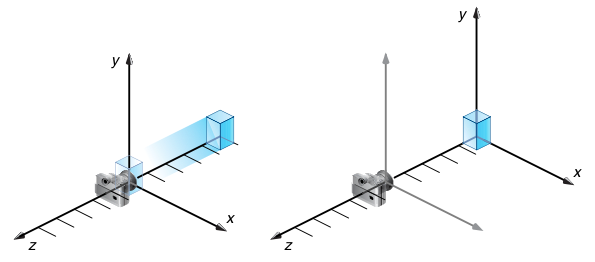
\includegraphics[width=300pt]{img/gltranslate.png}
    \caption{A view transformations by means of a glTranslate invocation}
    \label{fig:gltranslate}
  \end{center}
\end{figure}

\begin{figure}[ht]
  \begin{center}
    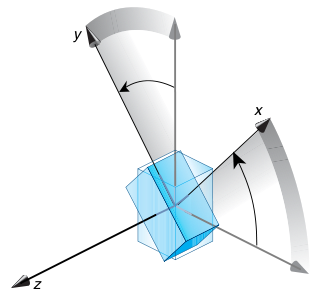
\includegraphics[width=150pt]{img/glrotate.png}
    \caption{A model transformation by means of a glRotate invocation}
    \label{fig:glrotate}
  \end{center}
\end{figure}
